\chapter{I Interviewed 30 Billionaires: What the Arithmetic Reveals}

This lecture from School of Hard Knocks, curated by LazyingArt LLC, begins by reversing the usual order of interrogation. The interviewer, who normally extracts principles from the wealthy, is himself made to answer for scale, method, and outcome. That inversion gives the lecture a real mathematical spine. We are not led into formal economics or finance, but into a sequence of business quantities, update rules, horizon choices, coverage arguments, and finally a stark arithmetic of finite time. What follows is a first-pass companion chapter that keeps close to the transcript and treats each equation as a disciplined reconstruction of the lecture's spoken logic.

\begin{remark}
No validated mathematical screenshots survive for this lecture. The figures in this chapter are therefore editorial reconstructions from the transcript, included only to clarify the structure of the spoken argument.
\end{remark}

\section{Opening inversion and the host as case study}

The lecture first manufactures authority through montage: celebrities, athletes, billionaires, and major entrepreneurs appear in quick succession. Then the structure flips. Instead of asking other people how they got rich, the host is asked to account for himself. That is the first important move. The speaker is no longer merely a collector of stories; he becomes a numerical example.

The host gives four scale markers that anchor the rest of the lecture:
\begin{align}
N_{\mathrm{B}} &> 30, &
N_{\mathrm{I}} &> 1000, \\
R_m &> \$700{,}000, &
R_y &> \$6{,}000{,}000.
\end{align}
Here \(N_{\mathrm{B}}\) is the number of billionaires interviewed over roughly four years, \(N_{\mathrm{I}}\) is the total interview count, \(R_m\) is recent monthly business revenue, and \(R_y\) is projected yearly business revenue.

The next question is exactly the right one: how can that sort of yearly revenue arise from an interview brand? The host answers by refusing a one-line story. He says that he does not merely create content; he has built several monetization channels around the core attention engine. A cautious reconstruction is
\begin{equation}
R = R_{\mathrm{agency}} + R_{\mathrm{consult}} + R_{\mathrm{brand}} + R_{\mathrm{ads}} + R_{\mathrm{sub}},
\end{equation}
where the right-hand side names the streams he actually lists: agency work, consulting, brand partnerships, ad revenue, and subscription or community revenue.

This is already one of the lecture's permanent ideas. Wealth at scale is not described as a single salary or even as a single business line. It is described as layered capture around a core asset.

\begin{figure}[h]
\centering
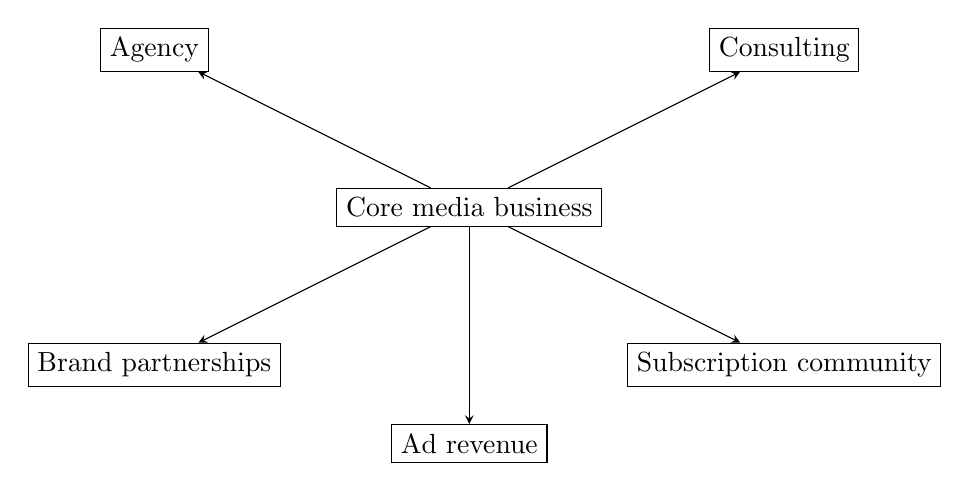
\begin{tikzpicture}[>=stealth]
\node[draw, rectangle] (core) at (0,0) {Core media business};
\node[draw, rectangle] (agency) at (-4,2) {Agency};
\node[draw, rectangle] (consult) at (4,2) {Consulting};
\node[draw, rectangle] (brand) at (-4,-2) {Brand partnerships};
\node[draw, rectangle] (ads) at (0,-3) {Ad revenue};
\node[draw, rectangle] (sub) at (4,-2) {Subscription community};

\draw[->] (core) -- (agency);
\draw[->] (core) -- (consult);
\draw[->] (core) -- (brand);
\draw[->] (core) -- (ads);
\draw[->] (core) -- (sub);
\end{tikzpicture}
\end{figure}

Once the speaker has supplied his own arithmetic, the guest raises the lecture's main challenge: compress more than a thousand interviews into fifteen lessons. That challenge gives the lecture its countdown rhythm. Each lesson arrives as a short clip, a restatement, and a harder operator claim. We should preserve that rhythm, because the lecture does not proceed as a single continuous proof. It proceeds by repeated compression.

\section{Advice, credibility, and the right to be heard}

The early ranks are not yet about scaling mechanics. They first establish an epistemic filter. Before we ask how to build, we ask whom we should listen to.

\paragraph{Anecdote.}
Will Smith gives the first sharp criterion: taking advice from someone who has not done what you want to do is a kind of madness. The host restates the point even more aggressively: do not take advice from someone you would not trade places with.

\begin{definition}
We shall call a piece of advice operationally admissible if the speaker has already done the thing being recommended.
\end{definition}

A compact way to write the rule is
\begin{equation}
\mathrm{admissible}(x) \Rightarrow x \text{ has already executed the target action.}
\end{equation}

That is not deep mathematics, but it is exact enough for the chapter. The lecture is building a filter on counsel. It is trying to reduce noise before it discusses mechanics.

The next lesson, from Robert Herjavec, attacks another piece of lazy folklore. The transcript is corrupted in the middle of this segment, so we should state the stable line only. The lecture rejects the slogan that success is mainly about already knowing the right people. Herjavec begins without family money or preloaded business access. The host's summary is the key: build some wins, establish your own credibility, and then serious people become reachable.

We can formalize the through-line as
\begin{equation}
\text{wins} \longrightarrow \text{credibility} \longrightarrow \text{access}.
\end{equation}

\begin{figure}[h]
\centering
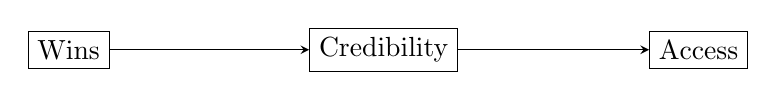
\begin{tikzpicture}[>=stealth]
\node[draw, rectangle] (wins) at (0,0) {Wins};
\node[draw, rectangle] (cred) at (4,0) {Credibility};
\node[draw, rectangle] (access) at (8,0) {Access};

\draw[->] (wins) -- (cred);
\draw[->] (cred) -- (access);
\end{tikzpicture}
\end{figure}

This matters for the lecture's architecture. The host is not merely saying that contacts matter less than skill. He is saying something more sequential: access is downstream of visible proof. That is why these lessons appear before the later sections on investing and scaling. One must first earn the right to be heard.

\section{Investing, retention, and the anti-consumption rule}

The next turn is from epistemology to capital. Ashley Fox supplies the lecture's clearest financial sentence: wealthy people do not leave money sitting still; they give it a job.

\subsection{Question \& Answer}

Can one save one's way to wealth? In the logic of this lecture, no. Mere saving adds what one contributes; investing adds both the new contribution and the return on the existing base. The lightest faithful formalization is
\begin{align}
W_{t+1}^{\mathrm{save}} &= W_t + s_t, \\
W_{t+1}^{\mathrm{invest}} &= (1+r_t)W_t + s_t.
\end{align}
Here \(W_t\) is wealth at time \(t\), \(s_t\) is new saving, and \(r_t\) is the return on deployed capital. The lecture is not deriving a finance model. It is marking the difference between additive accumulation and compounding accumulation. That difference is the entire point.

The lecture then breaks into a long promotional interlude about a live wealth-building event and a paid-access community. In final form this material should stay short, but it should not disappear. Structurally it shows that access to capital-allocation knowledge is itself treated as scarce and monetizable. Even the interruption obeys the lecture's logic: once investing is established as necessary, access to competent guidance becomes a product.

The Houston multimillionaire then gives the anti-consumption rule in its most memorable form: stay small enough, long enough, and you will be big enough soon enough. The arithmetic attached to the line matters. He says that he was making about \(\$30{,}000\) a month with roughly \(\$3{,}000\) to \(\$4{,}000\) in overhead, and that lifestyle expansion came only after millions had already been accumulated.

The host then sharpens the same rule by using his own early numbers. He says that when he and his partners were making about \(\$30{,}000\) a month in profit, they were paying themselves only about \(\$2{,}000\). The transcript is ambiguous about whether this draw is per partner or total, so the number must be used cautiously. Still, the operational point is plain: low draw preserves the machine.

A general retention rule is
\begin{equation}
K_{t+1} = K_t + \Pi_t - D_t + I_t,
\end{equation}
where \(K_t\) is retained business capital, \(\Pi_t\) is profit, \(D_t\) is owner draw, and \(I_t\) denotes deliberate reinvestment back into growth. If we suppress the bookkeeping distinction between retained profit and reinvestment, the anecdote becomes a worked example:
\begin{align}
\Delta K_m &= \Pi_m - D_m \\
&\approx \$30{,}000 - \$2{,}000 \\
&\approx \$28{,}000.
\end{align}

That is the lecture's real anti-consumption arithmetic. The point is not moral purity. The point is resilience. If the next month weakens, a thin lifestyle protects the firm. If the next month holds, retained capital compounds inside the operating system of the business.

\begin{figure}[h]
\centering
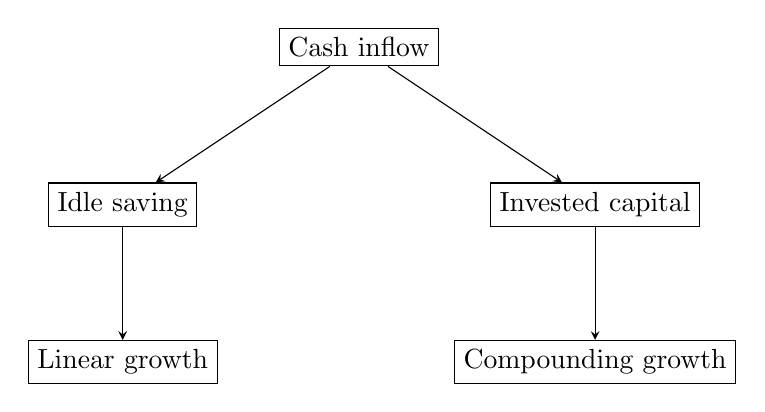
\begin{tikzpicture}[>=stealth]
\node[draw, rectangle] (income) at (0,2) {Cash inflow};
\node[draw, rectangle] (save) at (-3,0) {Idle saving};
\node[draw, rectangle] (invest) at (3,0) {Invested capital};
\node[draw, rectangle] (wealth1) at (-3,-2) {Linear growth};
\node[draw, rectangle] (wealth2) at (3,-2) {Compounding growth};

\draw[->] (income) -- (save);
\draw[->] (income) -- (invest);
\draw[->] (save) -- (wealth1);
\draw[->] (invest) -- (wealth2);
\end{tikzpicture}
\end{figure}

\section{Long horizons and omnipresence}

At rank eleven, the lecture moves from retention to horizon. Reid Hoffman is asked a very contemporary question: if one had to make a billion dollars in one year, what would one do? His answer is to reject the frame. He says that he almost never plays a one-year game; he plays a ten-year game.

This is one of the lecture's best changes of scale. Up to this point, we have seen monthly revenue, yearly revenue, and short-run consumption control. Hoffman widens the clock. The host compresses the lesson into a slogan: billionaires think in decades, not days.

We may write the contrast first as a simple inequality of frames:
\begin{equation}
T_{\mathrm{short}} = 1 \text{ year}, \qquad T_{\mathrm{long}} = 10 \text{ years}, \qquad T_{\mathrm{short}} \neq T_{\mathrm{long}}.
\end{equation}
But the lecture is really after the mechanism that becomes visible only on the longer horizon:
\begin{equation}
V_T = V_0 \prod_{t=1}^{T} (1+g_t).
\end{equation}
This is not a valuation formula quoted by the speaker. It is the canonical expression of what he means by compounding to ten years. If horizon extends, multiplicative growth begins to dominate additive thinking.

The next movement is from time-scale to distribution-scale. Mohammed Binghatti says that one must master sales and marketing and, more specifically, omnipresence. The business must be everywhere at once, or as close to that as resources allow. The host then translates the point into his own media experience: he says he has roughly three million followers on Facebook and makes more money there than on platforms where he has even larger followings. That is important. The lecture is distinguishing presence from vanity metrics.

A minimal formalization is
\begin{equation}
P = \sum_i p_i,
\end{equation}
where \(p_i\) measures effective presence on channel \(i\). The sum is not simply follower count. It is channel coverage weighted by commercial usefulness.

If the Hoffman lesson says that serious operators widen time, the Binghatti lesson says that serious operators widen surface area. One gives us horizon; the other gives us reach.

\section{Comfort, intelligence, and money while sleeping}

The next cluster changes the object of optimization. After one has learned to retain capital, think long, and distribute broadly, what disposition keeps the machine alive?

The ninth lesson comes from the entrepreneur who sold BodyArmor to Coca-Cola for eight billion dollars. The host's summary is concise and accurate: one may be happy without becoming content. Comfort, in this lecture, is a local equilibrium that invites predation. The language is harsh, but the logic is clear. Markets continue moving, competitors remain hungry, and inertia is punished.

The eighth lesson sharpens a different misconception. John Morgan, who became a billionaire through law, says he is not especially smart in the heroic sense. He is smart enough to know that he is not the expert in every domain, and smart enough to hire experts. The remembered line is the important one: ``I hire scientists.''

\subsection{Question \& Answer}

Does one need to be the smartest person in the room? The lecture's answer is no. What one needs is the capacity to recognize where intelligence is required, and then to place the right intelligence in the right role. The chapter should therefore resist the mythology of solitary genius. The operative function is coordination. Expertise is assembled, not mystically possessed in full by one founder.

The seventh lesson then carries the same demotion of brute labor into the domain of cash flow. Joshua Crisp gives the familiar line: if one cannot find a way to make money while sleeping, one will work until death. The host ties this back to the earlier investment section. Once more, wealth is not defined as effort alone. It is defined as a structure in which money, systems, or assets continue working when the founder is absent.

We should not formalize this too aggressively, because the lecture does not. Its point is operational, not actuarial. Labor-bound income may be necessary in the beginning. But the long-run target is clear: one moves from income that ceases when one stops, to income generated by capital, systems, or distribution that continue after the founder has stepped away.

\section{Change, marketing, speed, and the size of the game}

The last acceleration begins with Jim Keyes, former head of both 7-Eleven and Blockbuster. He gives the lecture's most explicit identity:
\begin{equation}
\text{Change} = \text{Opportunity}.
\end{equation}
Taken literally, that is an aphorism. Taken analytically, it says that environmental change is not valuable by itself. Value appears when one responds better than competitors. The more useful version is
\begin{equation}
\Delta E \longrightarrow A \longrightarrow V_{\mathrm{shareholder}},
\end{equation}
where \(\Delta E\) is a change in the environment, \(A\) is adaptive response, and \(V_{\mathrm{shareholder}}\) is the value created by reacting well when others resist.

Todd Johnson then makes the matching point about visibility. He says that many people need what one offers; they simply do not know who one is. This is the lecture's best statement on marketing: value hidden from the market may as well not exist. The host drives the point home by saying that one may have the ``magic sauce,'' but without leads and visibility there is no purchase.

The fourth lesson adds tempo. The Miami operator rejects procrastination entirely. In the lecture's logic, delay is not caution; it is often disguised fear. The host recasts this as an entrepreneurial rule: there is no perfect time, and success loves speed because markets penalize deferred action.

The third lesson then widens the target again.

\subsection{Question \& Answer}

Is a bigger game actually harder? The lecture answers with a provocative heuristic: the stress of solving \(\$1{,}000\) problems, \(\$10{,}000\) problems, \(\$100{,}000\) problems, and far larger problems may be less different than beginners imagine. The sequence given in the lecture is
\begin{equation}
\$10^3,\ \ \$10^4,\ \ \$10^5,\ \ \$10^6,\ \ \$10^7,\ \ \$10^8.
\end{equation}
The host's explanation is twofold. First, larger clients often possess more capital and therefore impose less desperate, penny-pinching pressure than very small clients. Second, competition is crowded at the bottom because almost everyone is trained to think small. A cautious formalization is
\begin{equation}
m_1 < m_2 \Rightarrow c(m_1) > c(m_2),
\end{equation}
where \(m\) is target problem size and \(c(m)\) is competition density.

This is not a theorem. It is an operator's heuristic. But it fits the lecture precisely. Think larger, and one may discover not only larger tickets, but cleaner air.

\begin{figure}[h]
\centering
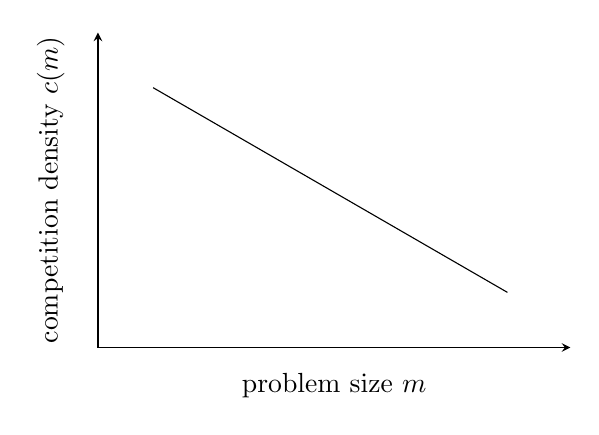
\begin{tikzpicture}[>=stealth]
\draw[->] (0,0) -- (6,0);
\draw[->] (0,0) -- (0,4);
\draw (0.7,3.3) -- (5.2,0.7);
\node[below] at (3,-0.2) {problem size \(m\)};
\node[rotate=90] at (-0.6,2) {competition density \(c(m)\)};
\end{tikzpicture}
\end{figure}

\section{Wings, ribbon, and the remaining interval}

The lecture's final two lessons are the strongest because they suddenly move beyond business. The countdown has been teaching us how to operate. Now it asks why operation matters at all.

Billy Ray Taylor first gives the bird-and-branch image. If a bird lands on a branch, does it trust the branch, or does it trust its wings? The host's interpretation is correct: the branch may fail, but the bird does not rely on the branch as the final source of safety. It relies on its own capacity to fly.

We may write the distinction very lightly:
\begin{equation}
\mathrm{trust}(\mathrm{branch}) \neq \mathrm{trust}(\mathrm{wings}).
\end{equation}
Again, this is not a literal formula from the speaker. It is the chapter's cleanest way of preserving the logical contrast. External supports matter, but they are not the true ground of confidence. The lecture's language is direct: believe in yourself, because no one else will do the believing for you.

The final lesson is the ribbon demonstration. Taylor imagines a strip marked from \(1\) to \(100\). He uses \(75\) and \(81\) as rough demonstration values for male and female lifespan, and then marks his current age, \(57\). The mathematical point is not actuarial precision. It is subtraction.

\subsection{Question \& Answer}

What exactly is left? In the first crude pass, if \(a\) is current age and \(L\) is a reference lifespan, then
\begin{equation}
L_{\mathrm{rem}} = L - a.
\end{equation}
Using the speaker's own demonstration values gives
\begin{align}
a &= 57, \\
L_{\mathrm{male}} &\approx 75, \\
L_{\mathrm{female}} &\approx 81,
\end{align}
and therefore
\begin{align}
L_{\mathrm{rem}}^{(75)} &\approx 18, \\
L_{\mathrm{rem}}^{(81)} &\approx 24.
\end{align}

But the lecture immediately adds the necessary caveat: late years do not necessarily have the same quality or mobility as early years. So the arithmetic alone is not the entire point. The ribbon is torn twice in thought. One part is already gone. Another part may exist only in diminished form. What remains is the interval one can actually act inside.

\begin{figure}[h]
\centering
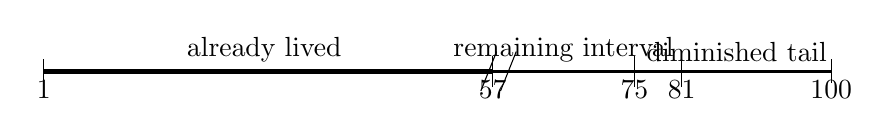
\begin{tikzpicture}[x=1cm,y=1cm]
\draw[line width=1pt] (0,0) -- (10,0);
\draw[line width=2pt] (0,0) -- (5.7,0);
\draw[dashed] (7.5,0) -- (10,0);

\draw (0,-0.15) -- (0,0.15);
\draw (5.7,-0.2) -- (5.7,0.2);
\draw (7.5,-0.2) -- (7.5,0.2);
\draw (8.1,-0.2) -- (8.1,0.2);
\draw (10,-0.15) -- (10,0.15);

\draw (5.55,-0.25) -- (5.75,0.25);
\draw (5.8,-0.25) -- (6.0,0.25);

\node[below] at (0,0) {1};
\node[below] at (5.7,0) {57};
\node[below] at (7.5,0) {75};
\node[below] at (8.1,0) {81};
\node[below] at (10,0) {100};

\node[above] at (2.8,0) {already lived};
\node[above] at (6.6,0) {remaining interval};
\node[above] at (8.8,0) {diminished tail};
\end{tikzpicture}
\end{figure}

That is why the lecture ends where it does. The final arithmetic is not about revenue, followers, deal size, or exits. It is about a finite interval that can no longer be rolled over. The line ``what you got left is what you got left'' is the countdown's last and most severe compression.

\section{Summary}

The lecture begins with authority, but it earns its chapter by turning authority into structure. First come scale markers: more than thirty billionaires, more than a thousand interviews, more than seven hundred thousand dollars in a month, more than six million in a year. Then come the operator rules: take advice only from those who have done the thing; build wins before asking for access; invest rather than merely save; retain capital before inflating lifestyle; think in decades; spread presence across channels; refuse comfort; hire intelligence; adapt to change; make value visible; act quickly; aim higher than the crowded bottom. Finally, the lecture collapses all business doctrine into a smaller frame: trust your wings, not the branch, and remember that the strip of time in front of you is not abstract. It is short, uneven, and already being consumed.

The mathematics of the lecture is therefore modest but real. It is the arithmetic of stacked revenue, compound horizons, retained capital, channel coverage, competitive density, and finite remaining life. That is enough structure to justify careful notes, and enough tension to support a later rewrite into a larger thematic book.